\documentclass[usenatbib,fleqn]{mnras}

\pdfoutput=1

\usepackage{amsmath}
\usepackage{amssymb}
% \usepackage{authblk}
\usepackage{balance}
\usepackage{bm}
% \usepackage[superscript,biblabel]{cite}
\usepackage{color}
% \usepackage{fullpage}
\usepackage{flushend}
\usepackage{graphicx}
\usepackage{hyperref}
% \usepackage[all]{hypcap}
\usepackage{lineno}
\usepackage{longtable}
\usepackage{multicol}
\usepackage{multirow}
\usepackage{natbib}
\usepackage{flushend}
% \usepackage{tablefootnote}
\usepackage{txfonts}
% \usepackage{unicode-math}
% \usepackage{wasysym}

\usepackage[capitalize,nameinlink]{cleveref}
% cleveref tweak to remove parentheses from equations
\creflabelformat{equation}{#2#1#3}
\crefrangelabelformat{equation}{#3#1#4 to #5#2#6}

% For links of references
\hypersetup{colorlinks,
  linkcolor=red,
  filecolor=red,
  urlcolor=magenta,
  citecolor=blue}

% define "struts", as suggested by Claudio Beccari in
%    a piece in TeX and TUG News, Vol. 2, 1993.
\newcommand\Tstrut[1]{\rule{0pt}{#1ex}}         % = `top' strut
\newcommand\Bstrut[1]{\rule[#1ex]{0pt}{0pt}}   % = `bottom' strut

\usepackage{array}
\newcolumntype{L}[1]{>{\raggedright\let\newline\\\arraybackslash\hspace{0pt}}m{#1}}
\newcolumntype{C}[1]{>{\centering\let\newline\\\arraybackslash\hspace{0pt}}m{#1}}
\newcolumntype{R}[1]{>{\raggedleft\let\newline\\\arraybackslash\hspace{0pt}}m{#1}}

\def\aap{A\&A}
\def\aaps{A\&AS}
\def\aapr{A\&ARv}
\def\aarv{A\&ARv}
\def\aj{AJ}
\def\ao{ApOpt}
\def\apj{ApJ}
\def\apjl{ApJL}
\def\apjs{ApJS}
\def\apss{Ap\&SS}
\def\araa{ARA\&A}
\def\aspc{ASPC}
\def\bjp{Braz.\ J.\ Phys.}
\def\casp{Comm.\ Astrophys.\ Space Phys.}
\def\helv{Helv.\ Phys.\ Acta}
\def\jcap{JCAP}
\def\mnras{MNRAS}
\def\nat{Nature}
\def\nature{Nature}
\def\njph{New.\ J.\ Phys.}
\def\obs{Observatory}
\def\pasa{PASA}
\def\pasp{PASP}
\def\physrep{Phys.\ Rep.}
\def\pnas{PNAS}
\def\prd{PhRvD}
\def\procspie{SPIE}
\def\ssr{Space Sci.\ Rev.}

/Users/cristobal/Documents/latex/macros/definitions.tex

% user definitions
\def\udg{\mathrm{UDG}}
\def\bound{\mathrm{bound}}
\def\Mcl{M_\mathrm{cl}}
\def\percent{ per cent}
\def\reff{r_\mathrm{eff}}


\title[Weak lensing masses of UDGs]{An upper limit on the masses of ultra diffuse galaxies from weak gravitational lensing}

\author[C.\ Sif\'on, R.\ F.\ J.\ van der Burg, H.\ Hoekstra, A.\ Muzzin \& R.\ Herbonnet]
  {
      Crist\'obal~Sif\'on$^{1,2}$,
      Remco~F.~J.~van~der~Burg$^3$,
      Henk~Hoekstra$^2$
      Adam~Muzzin$^4$
      and
      \newauthor
      Ricardo~Herbonnet$^2$
\\
      $^1$Department of Astrophysical Sciences, Peyton Hall, Princeton University, Princeton, NJ 08544, USA\\
      $^2$Leiden Observatory, Leiden University, PO Box 9513, NL-2300 RA Leiden, Netherlands\\
      $^3$Laboratoire AIM, IRFU/Service d'Astrophysique - CEA/DSM - CNRS - Universit\'e Paris Diderot, B\^at. 709, CEA-Saclay, 91191 Gif-sur-Yvette Cedex, France\\
      $^4$
  }

% \author[1,2]{Crist\'obal~Sif\'on}
% \author[3]{Remco~F.~J.~van~der~Burg}
% \author[4]{Adam~Muzzin}
% \author[2]{Henk~Hoekstra}
% \author[2]{Ricardo~Herbonnet}
% \affil[1]{Department of Astrophysical Sciences, Peyton Hall, Princeton University, Princeton, NJ 08544, USA}
% \affil[2]{Leiden Observatory, Leiden University, PO Box 9513, NL-2300 RA Leiden, The Netherlands}
% \affil[3]{Laboratoire AIM, IRFU/Service d’Astrophysique - CEA/DSM - CNRS - Universit\'e Paris Diderot, B\^{a}t. 709, CEA-Saclay, 91191 Gif-sur-Yvette Cedex, France}
% \affil[4]{York University}
% 
% % changes ", and" to " and". If you prefer ", and" then comment out
% \renewcommand\Authands{ and }
% \renewcommand\Authfont{\normalfont}
% \renewcommand\Affilfont{\small}


% These dates will be filled out by the publisher
% \date{Accepted XXX. Received YYY; in original form ZZZ}

% Enter the current year, for the copyright statements etc.
\pubyear{2016}

\begin{document}

\label{firstpage}
\pagerange{\pageref{firstpage}--\pageref{lastpage}}

\maketitle

\begin{abstract}
        The recent discovery of thousands of ultra diffuse galaxies (UDGs) in nearby galaxy clusters has opened a new window into the process of galaxy formation and evolution. Among the key features that could reveal their formation history and ability to survive in the harsh cluster environments are the masses of these UDGs. We use weak gravitational lensing measurements around 909 UDGs in 21 clusters at $z\leq0.09$ to constrain the average total mass of UDGs. We constrain the average mass of subhaloes hosting UDGs to $\log m_{\rm UDG}/\Msun\leq11.45$, within a radius $r\sim40$ kpc, at 95\percent\ confidence. Although uncertainties are large, our lensing measurements suggest that UDGs are dwarfs and not failed $L^*$ galaxies.
\end{abstract}

\section{Introduction}
\label{s:intro}

Large, low surface brightness galaxies have been known to exist both in the field \citep{} and in galaxy clusters \citep{} for some time. \textbf{their properties etc.}

A subset of these low surface brightness galaxies---dubbed ultra-diffuse galaxies (UDGs) by \cite{vandokkum15_coma}---has recently started receiving particular attention. UDGs stand out as the largest galaxies of their kind, with effective (of half-light) radii $\reff\geq1.5\,\mathrm{kpc}$, which are in fact typical of galaxies with masses similar to that of the Milky Way, $M\sim10^{12}\,\Msun$. In contrast, their stellar masses are only $\Mstar\lesssim10^8\,\Msun$. A striking feature of UDGs is the fact that they are a numerous population in massive galaxy clusters \citep{vandokkum15_coma,koda15,mihos15,yagi16,vdburg16}.

%\textbf{note however \cite{roman16}, who found UDGs all the way to filaments around A168.}
% While each cluster can host hundreds of UDGs, there are very few UDGs in the field \citep{vdburg16}, suggesting that their formation and evolution are intimately linked to the cluster environment.
Several hypotheses have been put forth to try to explain the unexpected survival of UDGs in massive clusters. In the initial discovery of UDGs in the Coma Cluster, \cite{vandokkum15_coma} suggested that UDGs may be failed $L^*$ galaxies which fell into the cluster at early times, after having used only a small fraction of their cold gas to form stars. Once part of a cluster, their remaining cold gas was removed and they were left as very dark matter dominated galaxies.
\cite{yozin15} have shown that such a mechanism can in fact produce UDG-like galaxies in hydrodynamical simulations.
Alternatively, \cite{amorisco16} and \cite{dicintio17} have suggested that the intrinsic properties of some dwarf galaxies are responsible for the formation of UDGs; they should therefore be abundant in the field. However, a study of UDGs in the field is complicated by the lack of redshift information, whereas large numbers of UDGs that happen to be co-located in projection with galaxy clusters can safely be assumed to be part of the cluster \citep[or at least a significant fraction of them; e.g.,][]{vdburg16}. Furthermore, the one UDG with a spectroscopic redshift has been confirmed to be part of the Coma cluster \citep{vandokkum15_spec}.

Among the properties of UDGs that may shed light on the models above and others, their total mass is a crucial one. Knowing the masses of UDGs would allow us to unambiguously rule out some classes of hypotheses as those summarized above, such as the `failed $L^*$' hypothesis. In fact, there have been some attempts at estimating the masses of individual UDGs. \cite{beasley16_virgo} measured a velocity dispersion of globular clusters associated with a UDG in the Virgo Cluster of $33_{-10}^{+16}\,\kms$ within 8.1 kpc, which suggests a virial mass\footnote{Note that subhaloes cannot be physically assigned a virial mass, since they are embedded in the potential of the host cluster. However, referring to virial masses offers a convenient point for comparison. We therefore adhere to the use of virial masses in this discussion, but adopt a different mass definition in our analysis (see \Cref{s:results}). See also the discussion in \citet{sifon17}.} $m_{200}\sim10^{11}\,\Msun$. Similar masses have been estimated for a few UDGs indirectly from the number of globular clusters \citep{beasley16_acs,peng16}. All these measurements suggest that UDGs are dwarf galaxies and not failed $L^*$ galaxies. On the other hand, \cite{vandokkum16} estimated a virial mass $m\sim10^{12}\Msun$ from the stellar velocity dispersion and globular cluster count of a particularly large UDG ($\reff=4.5\,\mathrm{kpc}$). Such mass is comparable to that of the Milky Way---possibly a failed $L^*$ galaxy. Since all of the above mass estimations refer to single UDGs, it is not clear how they can be interpreted in the context of the UDG population, and therefore they are of limited use in distinguishing UDG formation hypothesis. Instead, measurements of the masses of a representative population of UDGs are required to draw conclusions about their origin.


Only weak gravitational lensing---the distortion of light from background galaxies by the mass distribution of objects closer to us---can provide direct measurements of \emph{typical} masses of UDGs. In contrast to spectroscopic measurements of stellar velocity dispersion or globular cluster counts, lensing does not rely on faint, low-surface brightness baryonic tracers of the mass in galaxies. It therefore provides a clear advantage over stellar dispersion measurements or globular cluster counts. For instance, the globular clusters identified by \cite{beasley16_acs} have magnitudes $m_I\gtrsim26$ in the AB system, for a UDG \emph{in the Coma Cluster}. Evidently, such an analysis would be impossible for more distant objects. The feasibility of weak lensing for measuring the total masses of satellite galaxies has already been demonstrated \citep[e.g.,][]{sifon15_kids,sifon17,li16}.  

Here, we present the first direct constraints on the average masses of UDGs using measurements of weak lensing produced by UDGs in a sample of 21 clusters at $z<0.1$ taken from the Multi-Epoch Nearby Cluster Survey \citep[\meneacs][]{sand12}. Throughout this work we adopt a flat \lcdm\ model with $\Omega_\mathrm{m}=0.315$ and $H_0=70\,\mathrm{km\,s^{-1}Mpc^{-1}}$, consistent with the latest results of the \planck\ satellite \citep{planck15xiii}.

\section{Data analysis}
\label{s:data}


\subsection{UDG sample}

\begin{table}
 \centering
\caption{Cluster sample. Clusters masses, $M_{200}$, refer to the dynamical masses estimated by \citet{sifon15_cccp}, and $r_{200}$ are the radii containing such masses. Note that here the overdensity is defined with respect to the critical density of the Universe. The last two columns list the number of good UDG candidates after cleaning the sample by visual inspection, uncorrected for possible interlopers, and the estimated number of interlopers in parentheses.}
\label{t:clusters}
\begin{tabular}{l c r@{ $\pm$ }l c c}
\hline\hline
 \multirow{2}{*}{Cluster} & \multirow{2}{*}{Redshift} & \multicolumn{2}{c}{$M_{200}$} & $r_{200}$ & Number \\
         &          & \multicolumn{2}{c}{$(10^{14}\Msun)$} & $(\mathrm{Mpc})$ & of UDGs  \\[0.5ex]
\hline
%A85        & 0.055 & 10.2 & 1.8 & $2.0\pm0.1$ & \,\,\,97 \\
A119       & 0.044 &  7.4 & 1.2 & $1.8\pm0.1$ & \,\,\,82 \\
A133       & 0.056 &  5.5 & 1.6 & $1.7\pm0.2$ & \,\,\,78 \\
A399       & 0.072 &  6.6 & 2.0 & $1.8\pm0.2$ & \,\,\,63 \\
A401       & 0.074 &  8.9 & 2.3 & $1.9\pm0.2$ & \,\,\,57 \\
A780       & 0.055 &  7.2 & 2.7 & $1.8\pm0.2$ & \,\,\,57 \\
A1650      & 0.084 &  4.5 & 0.9 & $1.5\pm0.1$ & \,\,\,16 \\
A1651      & 0.085 &  8.0 & 1.3 & $1.9\pm0.1$ & \,\,\,35 \\
A1781      & 0.062 &  0.6 & 0.3 & $0.8\pm0.1$ & \,\,\,20 \\
A1795      & 0.063 &  5.0 & 0.9 & $1.6\pm0.1$ &      109 \\
A1991      & 0.059 &  1.9 & 0.5 & $1.2\pm0.1$ & \,\,\,35 \\
A2029      & 0.078 & 16.1 & 2.5 & $2.4\pm0.1$ & \,\,\,34 \\
A2033      & 0.080 &  7.7 & 2.0 & $1.8\pm0.2$ & \,\,\,25 \\
A2064      & 0.073 &  3.4 & 1.7 & $1.4\pm0.2$ & \,\,\,5 \\
A2065      & 0.072 & 14.4 & 2.5 & $2.3\pm0.1$ & \,\,\,19 \\
A2142      & 0.090 & 13.8 & 1.2 & $2.2\pm0.1$ & \,\,\,62 \\
A2495      & 0.079 &  4.1 & 0.8 & $1.5\pm0.1$ & \,\,\,13 \\
A2597      & 0.083 &  3.5 & 2.0 & $1.4\pm0.3$ & \,\,\,20 \\
A2670      & 0.076 &  8.5 & 1.2 & $1.9\pm0.1$ & \,\,\,26 \\
MKW3S      & 0.045 &  2.6 & 0.5 & $1.3\pm0.1$ & \,\,\,23 \\
ZWCL1215   & 0.077 &  7.7 & 1.7 & $1.9\pm0.1$ & \,\,\,33 \\

A85        & 0.055 & 10.2 & 1.8 & $2.0\pm0.1$ &      \,\,\,97 \\
A119       & 0.044 &  7.4 & 1.2 & $1.8\pm0.1$ &      \,\,\,82 \\
A133       & 0.056 &  5.5 & 1.6 & $1.7\pm0.2$ &      \,\,\,78 \\
A399       & 0.072 &  6.6 & 2.0 & $1.8\pm0.2$ &      \,\,\,63 \\
A401       & 0.074 &  8.9 & 2.3 & $1.9\pm0.2$ &      \,\,\,57 \\
A780       & 0.055 &  7.2 & 2.7 & $1.8\pm0.2$ &      \,\,\,57 \\
A1650      & 0.084 &  4.5 & 0.9 & $1.5\pm0.1$ &      \,\,\,16 \\
A1651      & 0.085 &  8.0 & 1.3 & $1.9\pm0.1$ &      \,\,\,35 \\
A1781      & 0.062 &  0.6 & 0.3 & $0.8\pm0.1$ &      \,\,\,20 \\
A1795      & 0.063 &  5.0 & 0.9 & $1.6\pm0.1$ &           109 \\
A1991      & 0.059 &  1.9 & 0.5 & $1.2\pm0.1$ &      \,\,\,35 \\
A2029      & 0.078 & 16.1 & 2.5 & $2.4\pm0.1$ &      \,\,\,34 \\
A2033      & 0.080 &  7.7 & 2.0 & $1.8\pm0.2$ &      \,\,\,25 \\
A2064      & 0.073 &  3.4 & 1.7 & $1.4\pm0.2$ & \,\,\,\,\,\,5 \\
A2065      & 0.072 & 14.4 & 2.5 & $2.3\pm0.1$ &      \,\,\,19 \\
A2142      & 0.090 & 13.8 & 1.2 & $2.2\pm0.1$ &      \,\,\,62 \\
A2495      & 0.079 &  4.1 & 0.8 & $1.5\pm0.1$ &      \,\,\,13 \\
A2597      & 0.083 &  3.5 & 2.0 & $1.4\pm0.3$ &      \,\,\,20 \\
A2670      & 0.076 &  8.5 & 1.2 & $1.9\pm0.1$ &      \,\,\,26 \\
MKW3S      & 0.045 &  2.6 & 0.5 & $1.3\pm0.1$ &      \,\,\,23 \\
ZWCL1215   & 0.077 &  7.7 & 1.7 & $1.9\pm0.1$ &      \,\,\,33 \\
[0.5ex]
\hline
\end{tabular}
\end{table}

\meneacs\ is a multi-epoch survey of 57 clusters at $z\leq0.15$ carried out with Megacam in the Canada-France-Hawaii Telescope \citep{sand12}. The data reduction is described in detail by \cite{vdburg13,vdburg16}. The resulting full width at half maximum of the point spread function is less than 1 arcsec for all clusters in the sample, and the photometric zero points have been calibrated to about 0.01 mag.
%
We consider 21 of those 57 clusters, located at $z\leq0.09$, where we can still identify most UDGs given their surface brightness. These clusters have masses $M_{200}\gtrsim10^{14}\,\Msun$, as determined from galaxy velocity dispersions \citep{sifon15_cccp}. We list our cluster sample in \Cref{t:clusters}.

Following the original definition by \cite{vandokkum15_coma}, \cite{vdburg16} identified UDGs in a subset of our clusters as galaxies with surface brightnesses within one effective radius of $24.0\leq \langle\mu(r,\reff)\rangle\leq26.5$ and effective radii $1.5\leq\reff/\mathrm{kpc}\leq7.0$; these parameters were measured with \galfit\ \citep{peng02,peng10}. In order to have a sample that is as pure as possible but still obtain a large enough number of UDG candidates, \cite{vdburg16} considered eight clusters at $0.044\leq z \leq0.063$ and at galactic latitude $b\geq25^\circ$. The study of \cite{vdburg16} is unique in that they did not select UDGs by visual inspection after the automatic selection based on structural parameters. While this has the disadvantage that the sample may be (and in fact is, as we show below) contaminated by artefacts of various kinds, it allows for an objective, statistically-consistent study of their properties after accounting for the expected number of such objects in control fields. This contamination however can significantly alter lensing measurements in a way that may not be fully captured by subtracting the signal from a control sample.

We therefore start from the sample compiled by \cite{vdburg16}, but take some additional steps to define the sample used for weak lensing measurements. We first expand the cluster sample to $z\leq0.09$ in order to increase the number of UDGs in our sample. We also impose stricter size cuts on the UDG sample $\reff\geq2.0\,\mathrm{kpc}$ for $z\leq0.065$ and $\reff\geq3.0\,\mathrm{kpc}$ for higher redshifts, as we find that these cuts significantly reduce the contamination of the sample. Finally, we visually inspected all UDG candidates and only kept high-confidence UDG candidates. We classify a UDG candidate as high-confidence if it does not suffer significant blending with other galaxies; this ensures that the measured structural parameters are unbiased (i.e., without significant residuals in a model-subtracted image), but do not make any visual selection based on surface brightness, color or morphology. While this somewhat subjective selection could potentially bias statistical analyses such as that carried by \cite{vdburg16}, it is essential for a clean interpretation of lensing measurements around the UDGs. We show the distribution of stellar mass of our final sample of UDGs in \Cref{f:hist}.

\begin{figure}
 \centerline{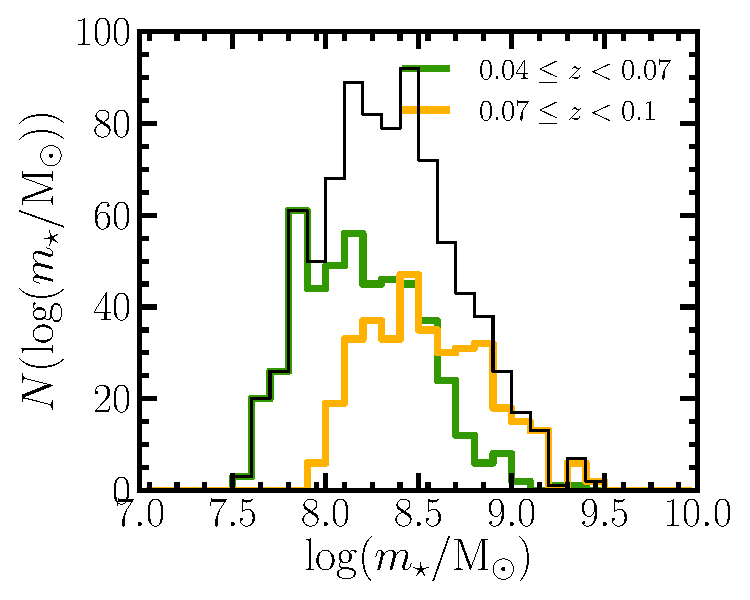
\includegraphics[width=0.8\linewidth]{logmstar_redshift.pdf}}
 \centerline{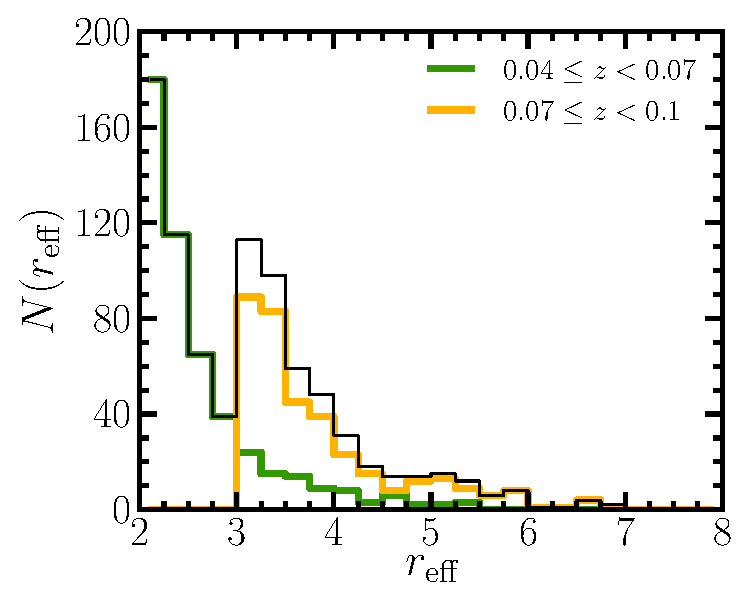
\includegraphics[width=0.8\linewidth]{reff_redshift.pdf}}
\caption{Distribution of stellar masses (top) and effective radii (bottom) of the UDG candidates that pass our visual inspection, split into a low (green) and high (orange) redshift samples. The thin black lines show the distribution for the full sample.}
\label{f:hist}
\end{figure}


\subsection{Weak lensing measurements}

Our weak lensing analysis is identical in methodology to that presented in \cite{sifon17}, which follows closely the cluster lensing analyses of \cite{hoekstra15} and Herbonnet et al.\ (in prep.). The weak lensing signal is measured as an average tangential alignment, or shear, $\gammat$, of galaxies in the background of the lenses (in this case, UDGs) using the moments-based KSB algorithm \citep{kaiser95,luppino97,hoekstra98}. The shear is closely related to the excess surface density, $\esd$, 
\begin{equation}
 \esd \equiv \bar\Sigma(<R) - \bar\Sigma(R) = \sigmac\gammat,
\end{equation}
where $\bar\Sigma(<R)$ and $\bar\Sigma(R)$ are the average surface densities within a projected radius\footnote{As a convention, we list two-dimensional distances with upper case $R$ and three-dimensional distances with lower case $r$.} $R$ and within a thin shell around $R$, respectively, and $\sigmac$ is a geometric factor accounting for the lensing efficiency,
\begin{equation}
 \sigmac \equiv \frac{c^2}{4\pi G} \frac{D_\mathrm{s}}{D_\mathrm{l}D_\mathrm{ls}},
\end{equation}
with $D_\mathrm{s}$, $D_\mathrm{l}$ and $D_\mathrm{ls}$ being the angular diameter distances to the source, to the lens, and between the lens and the source.

We define our source sample in an identical way to \cite{sifon17}. We do not apply any colour cuts to the sample, but correct the lensing measurements with a `boost factor' that accounts for contamination by cluster members. This boost factor has been calibrated using tailor-made image simulations in which each the red sequence galaxies of each cluster have been added to a simulation of the background source population, reproducing the noise and seeing properties of the real data (Herbonnet et al.\ in prep.). These simulations also allow us to assess obscuration of background galaxies by cluster galaxies, which biases the determination of the boost factor. In \cite{sifon17}, we found a significant obscuration by typical satellite galaxies galaxies at scales $R\lesssim20$ kpc. UDGs, however, have low surface brightness and do not produce any significant obscuration; instead we calculate the average obscuration as a function of cluster-centric distance, as in Herbonnet et al.\ (in prep.), to correct the boost factor. We also find that the tangential additive bias on the lensing measurements due to extended lens light, found to be about 30\% at $R\sim20$ kpc for typical satellites by \citep{sifon17}, is negligible for UDGs.


\section{The weak lensing signal of Ultra Diffuse Galaxies}
\label{s:results}

\subsection{Model for the UDG lensing signal}

As described in detail in \cite{yang06} and \cite{sifon15_kids}, the satellite lensing signal can be described by the sum of a subhalo and a host halo terms, both of which are essentially independent of each other. We model the average density profile of both UDGs and the host clusters as NFW profiles \citep{nfw95}.
% ,
% \begin{equation}\label{eq:nfw}
%  \rho(x) = \frac{\delta_\mathrm{c}\rho_\mathrm{m}}{x\,(1+x)^2},
% \end{equation}
% where $x \equiv r/\rs$, with $\rs$ the scale radius, and $\rho_\mathrm{m}=3H_0^2(1+z)^3\Omega_\mathrm{m}/(8\pi G)$ is the mean density of the Universe at redshift $z$. In addition, $\delta_\mathrm{c}$ is a function of the concentration, $c$,
% \begin{equation}
%  \delta_\mathrm{c}=\frac{200}{3}\frac{c^3}{\ln(1+c)-c/(1+c)}.
% \end{equation}
%
Following \cite{sifon17}, we define the mass of subhaloes hosting UDGs, $m_\mathrm{bound}$, as the bound subhalo mass---that is, the mass within the region where the density is above the background density of the cluster. In order to estimate the background density, we take the expected value for the three-dimensional radius based on the number density profile of normal cluster galaxies measured by \cite{vdburg15}, which provides a good description of the distribution of UDGs outside $R_\mathrm{sat}\sim0.15\radius$. Specifically,
\begin{equation}
 \langle r_\mathrm{UDG} \rangle = 
%   \frac{\int_{0.15}^c \mathrm{d}x' x'\,\rho(x', c)}{\int_{0.15}^c \mathrm{d}x' \rho(x', c)},
  \left[\int_{0.15c}^c d\chi\,\rho(\chi, c)\right]^{-1}
    \int_{0.15c}^c d\chi\,\chi\,\rho(\chi, c) = 0.38r_\mathrm{200,h}\,,
\end{equation}
where $\rho(x, c)$ is the NFW profile, with an adopted $c=2$ for satellite galaxies (including UDGs) in \meneacs\ clusters \citep{vdburg15,vdburg16}.
Our model therefore has four parameters: the average masses and concentrations of UDGs and the corresponding ones for host clusters. In practice, we are only able to constrain the masses of UDGs and their host clusters; we treat the concentrations as nuisance parameters.

We fit this model to the measurements using the affine-invariante Markov Chain Monte Carlo (MCMC) ensemble sampler \texttt{emcee} \citep{foreman13}, fully accounting for the data covariance as described in \cite{sifon15_kids,sifon17}. We adopt flat priors for all parameters in the following ranges:
\begin{equation}
\begin{split}
  8.5 &\leq \log(m_\mathrm{200,UDG}/\Msun) \leq 13.0 \\
 14.0 &\leq \log(M_\mathrm{200,cl}/\Msun) \leq 16.0 \\
   10 &\leq c_\mathrm{UDG} \leq 20 \\
    2 &\leq c_\mathrm{cl} \leq 8
 \,.
\end{split}
\end{equation}



\subsection{Constraints on the average UDG mass}

\begin{figure}
 \centerline{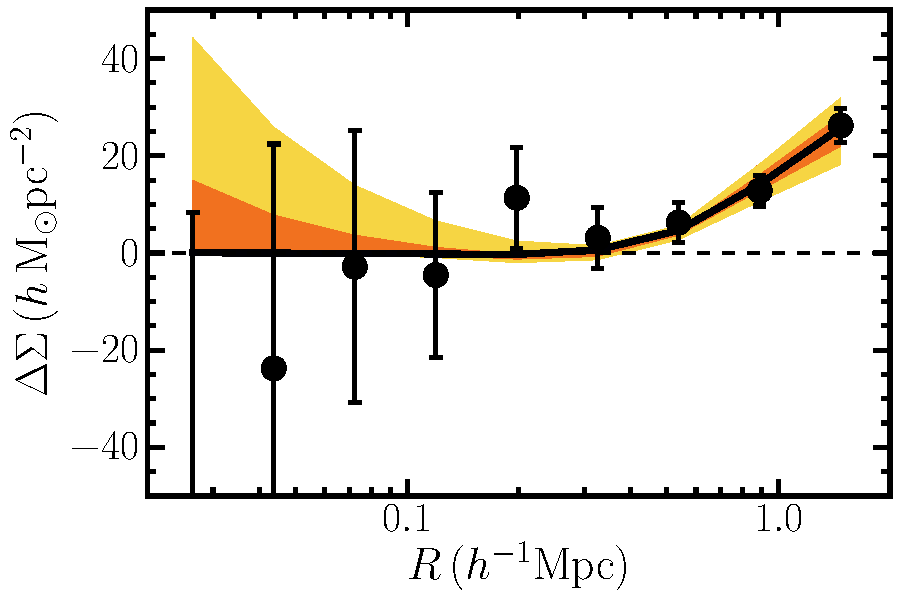
\includegraphics[width=0.95\linewidth]{esd.pdf}}
\caption{Lensing signal of ultra-diffuse galaxies in clusters at $z\leq0.09$. Orange and yellow regions show the 68 and 95\percent\ credible intervals from the MCMC sampling, while the black line shows the best-fit model.}
\label{f:esd}
\end{figure}

% \begin{figure}
%  \centerline{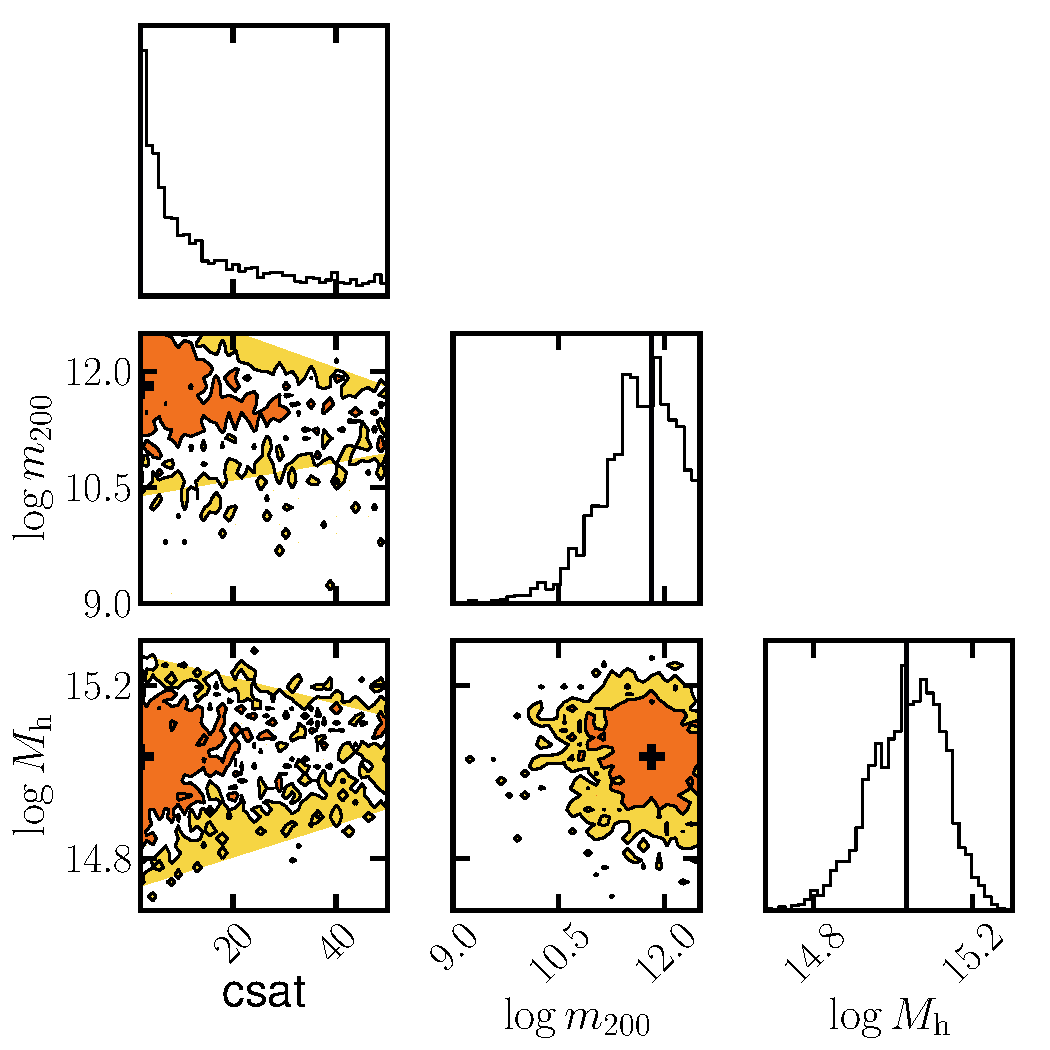
\includegraphics[width=0.95\linewidth]{corner.pdf}}
% \end{figure}

We show in \Cref{f:esd} the lensing signal of our sample of UDGs, along with the best-fit model. For UDGs we use a range $10 \leq c_\udg \leq 20$, which covers the expected average concentrations of subhaloes in the mass range $\log m/\Msun \sim 10-12$ and at cluster-centric distances $0.1\lesssim r/r_\mathrm{200,cl} \lesssim 1$ \citep{moline16}. Similarly, we set $2 \leq c_\mathrm{cl} \leq 8$ for the host clusters \citep[e.g.,][]{dutton14}.

Our model constrains the `virial' mass of subhaloes to $\log m_{200}/\Msun\leq11.94$ at 95\percent\ credibility. At an average cluster-centric distance of $\langle r_\udg \rangle=0.38r_\mathrm{200,cl}$, this results in a bound mass $\log m_\bound/\Msun\leq 11.45$ within a radius $r_\bound=41_{-37}^{+41}\,\mathrm{kpc}$ at 95\percent\ credibility. The wide range in $r_\bound$ is given by the range in allowed host cluster masses, which changes both the background density and the value of $r_\mathrm{200,cl}$. The best-fit host cluster mass is $\log\Mcl/\Msun=14.96_{-0.11}^{+0.11}$ (68\percent\ credible interval).

These results are somewhat dependent on the range chosen for $c_\udg$, with lower concentrations allowing for higher subhalo masses. However, it is unlikely that subhaloes would have concentrations much lower than $c=10$---these are in fact the typical concentrations of \emph{host} haloes of these masses \citep[e.g.,][]{dutton14,moline16}.

To allow a comparison with recent measurements of UDG masses from stellar dynamics and globular clusters, we also report the upper limit for the mass within 10 kpc, $m_\mathrm{<10\,kpc}\leq XX\,\Msun$, but we note that this value is an extrapolation of the data---a result of the adopted NFW profile.

% \begin{table}
% \begin{tabular}{l c c c c}
% \hline\hline
% \multirow{2}{*}{Parameter} & \multirow{2}{*}{Symbol} & \multirow{2}{*}{Units} & Prior & Posterior \\
%   &  &  & range & value \\
% \hline
% UDG mass
% \end{tabular}
% \end{table}


\section{Discussion}
\label{s:discussion}
 
Weak gravitational lensing measures the total mass irrespective of its nature. The median stellar mass of UDGs in our sample is $\langle m_\star \rangle = 2.0\times10^8\,\Msun$. Thus their dark matter fraction can be as high as 99.9\percent, although we are not able to detect mass in excess of the stellar mass. Lensing has the advantage compared to stellar dynamics that it probes the total masses of galaxies, instead of the masses within the small radii within which velocity dispersions can be measured \citep[e.g., roughly 8 kpc in the case of DF17 in the Coma cluster][]{beasley16_acs,peng16}, and therefore allows a more straightforward comparison with other kinds of galaxies, without the need for an extrapolation of the density profile from $\sim8$ kpc to tens of kpc (although lensing also relies to some extent on an assumed density profile).

However, weak lensing has therefore the disadvantage that the total and stellar masses are measured at very different radii, and the question of how dark matter--dominated these galaxies are, compared to dwarf or `normal' galaxies, is difficult to address.

Our weak lensing measurements suggest the typical UDG (with $\langle\reff\rangle\sim3$ kpc) resides in a dark matter halo that contains at most half the mass of the Milky Way. This supports the idea that UDGs are dwarfs, as opposed to failed $L^*$ galaxies. This is in agreement with the mass suggested by globular cluster counts in a $\reff=2.5\,\mathrm{kpc}$ UDG in the Coma cluster \citep{beasley16_acs,peng16}. On the other hand, \cite{vandokkum16} estimated a virial mass of about $10^{12}\,\Msun$ for DF44 (also in Coma). This UDG has a stellar mass $m_\star\sim3\times10^8\,\Msun$, similar to the average stellar mass in our sample, but an effective radius $\reff\sim4.5\,\mathrm{kpc}$, not representative of UDGs in general. The total mass inferred by \cite{vandokkum16} suggests either that DF44 is an outlier, \emph{compared to the population of UDGs}, in terms of its total-to-stellar mass ratio, or that the assumed extrapolation from a dynamical mass of $7\times10^9\,\Msun$ within 4.6 kpc to a virial mass of $\sim10^{12}\,\Msun$ is not valid. For this extrapolation, \cite{vandokkum16} assumed a concentration of $c\sim10$ \citep{maccio08}, at the low end of our chosen range. As discussed above, lowering the concentration tends to increase the mass allowed by our lensing measurements, and this may partly explain the fact that we consider DF44 an outlier. A study of the velocity dispersion of a statistical sample of UDGs may help understand this difference.

Our upper limit on the mass of UDGs suggests that they are not strong outliers in the total-to-stellar mass relation of cluster galaxies, as measured by \cite{sifon17}. So far, theoretical scenarios in which UDGs are dwarf galaxies also require an abundant field UDG population. A study of field UDGs would face the additional challenge that it would be very difficult to determine their redshifts in large numbers.

\textbf{make plot like right panel of fig 8 with the UDG upper limit}


% \balance

\bibliographystyle{mnras}
\bibliography{bibliography}

\end{document}
